\section{Qualifying the 737 ClaudeNet v2 sweep candidates}
A campaign to test whether any of the 737 new-and-unseen DR9-sweep candidates (group-conformal FDR$\le$0.05) could be genuinely undiscovered strong lenses, via an expanded crossmatch (SIMBAD + DES/KiDS VizieR; NED/SuGOHI unreachable) and two methodologically-independent visual passes: a structured Huang-VI rubric pass with an adversarial skeptic re-check, and the independent \texttt{lensjudge} harness (factored multiagent, Claude-opus). \emph{Qualified} = still NEW after the crossmatch AND graded A/B by BOTH passes.
\par\medskip\noindent\textbf{Result.} Of 737 candidates, 136 (18\%) coincide with a known lens or lens-candidate (92 DES, plus KiDS and SIMBAD lens-types); \textbf{601} remain NEW. \emph{None} of the 601 new candidates is graded A/B by either grader's strongest pass, so \textbf{qualified $=0$}. This is not the graders rejecting everything: together they graded 5 candidates $\ge$B, and \textbf{all 5 are already-catalogued lenses} (4 sub-arcsecond DES matches) --- the consensus re-discovered real lenses and found nothing comparable among the new ones.
\par\medskip\noindent\emph{Lenses the campaign re-discovered (already catalogued; the validation):}
\begin{figure}[t]\centering
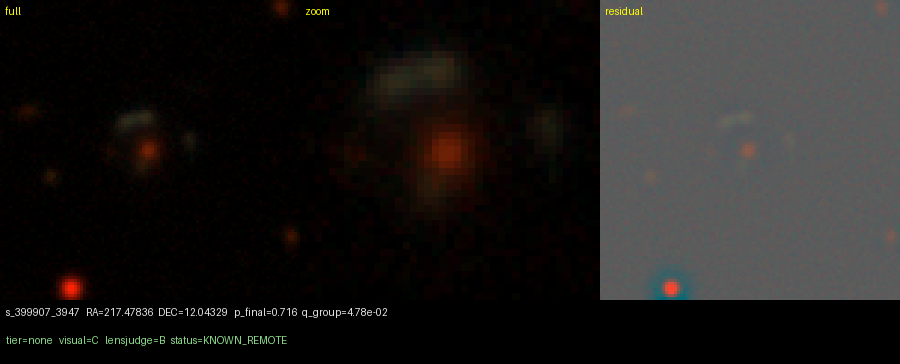
\includegraphics[width=0.92\textwidth]{../campaign/report/figs/recovered_01_s_399907_3947.png}
\caption{\textbf{s\_399907\_3947}: RA=217.47836, DEC=12.04329, $p_{\rm final}$=0.716; status KNOWN\_REMOTE (nearest curated at 6464.70$''$); visual C, lensjudge B. Full $|$ zoom $|$ residual.}
\end{figure}
\begin{figure}[t]\centering
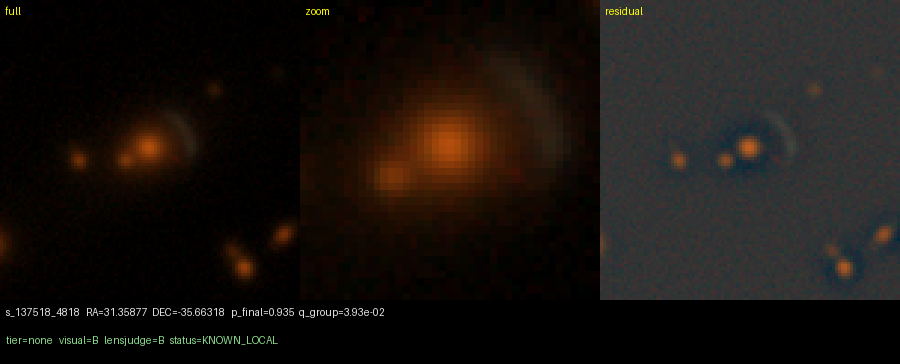
\includegraphics[width=0.92\textwidth]{../campaign/report/figs/recovered_02_s_137518_4818.png}
\caption{\textbf{s\_137518\_4818}: RA=31.35877, DEC=-35.66318, $p_{\rm final}$=0.935; status KNOWN\_LOCAL (nearest des\_jacobs2019 at 0.14$''$); visual B, lensjudge B. Full $|$ zoom $|$ residual.}
\end{figure}
\begin{figure}[t]\centering
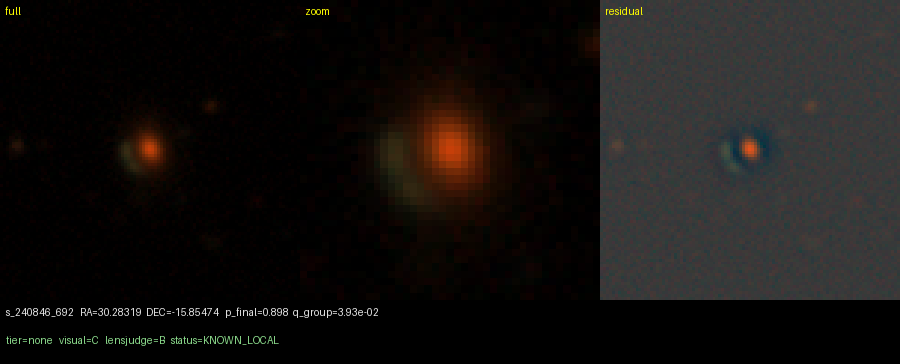
\includegraphics[width=0.92\textwidth]{../campaign/report/figs/recovered_03_s_240846_692.png}
\caption{\textbf{s\_240846\_692}: RA=30.28319, DEC=-15.85474, $p_{\rm final}$=0.898; status KNOWN\_LOCAL (nearest des\_jacobs2019 at 0.05$''$); visual C, lensjudge B. Full $|$ zoom $|$ residual.}
\end{figure}
\begin{figure}[t]\centering
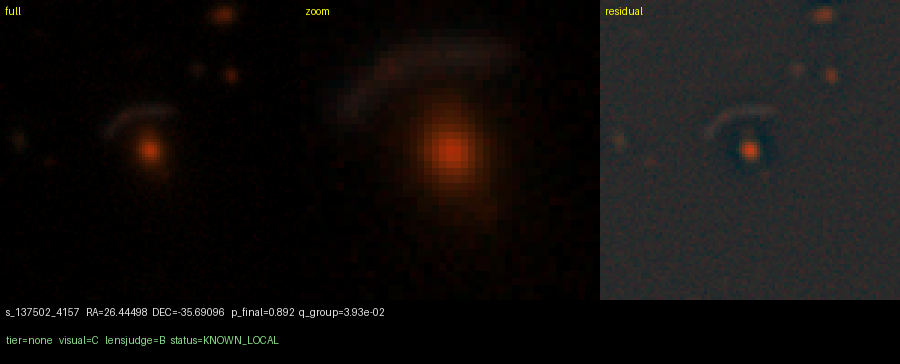
\includegraphics[width=0.92\textwidth]{../campaign/report/figs/recovered_04_s_137502_4157.png}
\caption{\textbf{s\_137502\_4157}: RA=26.44498, DEC=-35.69096, $p_{\rm final}$=0.892; status KNOWN\_LOCAL (nearest des\_jacobs2019 at 0.19$''$); visual C, lensjudge B. Full $|$ zoom $|$ residual.}
\end{figure}
\begin{figure}[t]\centering
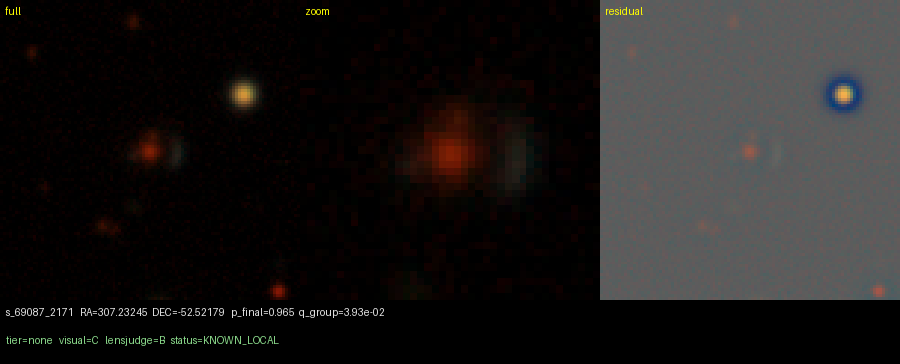
\includegraphics[width=0.92\textwidth]{../campaign/report/figs/recovered_05_s_69087_2171.png}
\caption{\textbf{s\_69087\_2171}: RA=307.23245, DEC=-52.52179, $p_{\rm final}$=0.965; status KNOWN\_LOCAL (nearest des\_jacobs2019 at 0.09$''$); visual C, lensjudge B. Full $|$ zoom $|$ residual.}
\end{figure}
